%!TEX root = ../tesi.tex

\chapter{Lo Shadow Framework 2.0}
\label{ch:shadowframework}
Questo capitolo presenta inizialmente una panoramica sugli attuali sistemi per la realizzazione di applicazioni che fanno uso di grafica tridimensionale real-time. Successivamente viene presentato lo ShadowFramework 2.0, le sue caratteristiche, la sua struttura e i suoi sviluppi futuri.

\section{Panoramica sui framework per la grafica 3D interattiva}
\label{sec:panoramicastrumenti}
Lo scopo della presente tesi di laurea \`e quello di produrre dei moduli di estensione per lo Shadow Framework, utili alla realizzazione di applicativi 3D orientati al web. 
Per lo stesso scopo esistono sul mercato una grande quantit\`a di soluzioni le cui caratteristiche possono essere notevolmente differenti in base al target di sviluppo a cui si rivolgono.

Prima di fornire una descrizione di alcune di queste soluzioni \`e bene introdurre alcuni concetti utili a comprendere quali sono i punti focali che distinguono un prodotto da un altro. L'elemento fondamentale di ognuno di questi questi software \`e l'\textbf{engine}, altrimenti detto rendering engine o 3D-engine. Questo \`e il nucleo di ogni programma grafico e fornisce una serie di meccanismi che, sfruttando le \ac{API} di programmazione grafica, permettono di disegnare su schermo i modelli tridimensionali voluti. Quando un prodotto consiste nel solo engine viene fornito nella forma di una libreria con cui \`e possibile interagire attraverso una \ac{API} specifica e che permette di configurare i passaggi della fase di rendering.

Dato che la pi\`u grande fetta di mercato per queste soluzioni software proviene dallo sviluppo di videogames sono nati una serie di software definiti \textbf{game engine}, questi sono veri e propri framework per la produzione di applicazioni 3D e, oltre al rendering engine, integrano al loro interno moduli per la gestione della fisica, del suono, delle animazioni e di tutte quelle componenti utili per lo sviluppo di giochi per computer. Questi framework possono essere forniti sia sotto forma di libreria da integrare nel proprio codice che con tool grafici che permettono di creare la propria applicazione da zero, utilizzando solamente gli strumenti forniti.

Seguendo questa classificazione e dato che l'intento dello Shadow Framework \`e fornire un set di librerie completo per la creare applicazioni grafiche, con moduli per gestire animazioni e dati oltre che alla semplice renderizzazione, senza per\`o vincolare all'utilizzo di librerie specifiche per elementi come l'intelligenza artificiale, il suono o altro che non sia direttamente coinvolto nella gestione della grafica, esso si trova a met\`a strada tra un rendering engine puro e un game engine.

Vengono ora presentati alcuni dei prodotti presenti sul mercato, la scelta di quali di essi presentare rispetto ad altri che non verranno citati non riflette la loro qualit\`a, ma \`e stata fatta su base rappresentativa.

% TODO: inserire i simboli di copyright ecc
\subsection{Game engine per Adobe Flash}
In questo caso invece che un prodotto specifico si preferisce citare una categoria di software. Per l'ambiente di Adobe esistono una grande quantit\`a di game engine che sfruttano le \ac{API} Flash per effettuare il rendering dei contenuti. Sebbene questo framework venga utilizzato da molti anni per la realizzazione di applicativi e che per lungo tempo abbia rappresentato l'ambiente di riferimento per applicativi web 3D, solo dalla release 11 comincia a sfruttare l'accelerazione hardware per la grafica tridimensionale.

Attualmente l'accelerazione consente di sfruttare le GPU a pipeline programmabile, ma non consente di usare le modalit\`a legacy a pipeline fissa. 
Inoltre non vengono rese disponibili le \ac{API} grafiche per la programmazione nativa come OpenGL o DirectX, ma una \ac{API} proprietaria di nome Stage3D che fornisce un'astrazione di livello pi\`u alto e semplifica la gestione delle risorse.
Questo sebbene consenta di semplificare e unificare tutte le piattaforme compatibili rende necessarie delle limitazioni per conservare la compatibilit\`a, rendendo inaccessibili le funzionalit\`a pi\`u avanzate degli hardware moderni (ad esempio \`e supportato lo Shader Model solo fino alla versione 2.0 sebbene oggi sia disponibile la versione 5.0).
Questi dati sono reperiti da \cite{site:adobestage3d}.

\subsection{Unity 3D}
Unity 3D \`e un game engine completo che dal 2005 ad oggi ha accresciuto molto la sua popolarit\`a. Uno dei maggiori punti di forza di questo ambiente consiste nella presenza di una discreta quantit\`a di tool grafici integrati tra loro, per il controllo del workflow di sviluppo. Sono inoltre integrati molti moduli per controllare aspetti quali le animazioni, la verifica delle performance ed il networking.
Un qualit\`a di primo piano \`e la compatibilit\`a di un elevato numero di piattaforme, consentendo di pubblicare le applicazioni realizzate su piattaforme mobile (android e iOS), desktop (Windows, Mac e Linux), console e web (via browser).
A proposito di quest'ultimo caso la fruizione dei contenuti via web \`e effettuata con due diversi metodi: o tramite un player flash o tramite l'\ac{API} Google Native Client del browser Chrome che permette l'esecuzione di codice nativo all'interno del browser.
In generale Unity 3D \`e un game engine moderno con pieno supporto alle ultime tecnologie grafiche rendendolo uno prodotto molto rappresentativo.
Oltre alle caratteristiche citate buona parte del suo successo \`e probabilmente dovuto alla grande comunit\`a di sviluppatori, anche indipendenti, ed alla numerosa quantit\`a di asset grafici disponibili.

\subsection{Unreal Engine e Unigine engine}
Entrambi questi prodotti sono game engine completi piuttosto famosi per l'elevatissima qualit\`a delle loro capacit\`a di rendering. Entrambi vengono infatti spesso utilizzati come benchmark per testare le capacit\`a grafiche hardware. Entrambi questi progetti sono maturi e moderni essendo dotati di tool grafici specifici e supportando le pi\`u recenti architetture grafiche. Entrambi supportano la maggior parte delle piattaforme desktop, mobile e consolle. Sebbene l'Unreal engine supporti anche flash e l'Unigine no, sono presentati insieme in quanto esempio di nuovo approccio alla distribuzione via web: entrambe le compagnie produttrici di questi software stanno infatti investendo nel portare i loro framework a supportare \ac{API} WebGL. Gli annunci ufficiali possono essere trovati a questi riferimenti \cite{site:mozillaunrealannounce,site:unigineannounce}.

\subsection{OnLive e Gaikai}
I due citati nel titolo non sono software per produrre applicazioni di grafica, ma due servizi a pagamento per la fruizione di applicazioni e videogiochi attraverso lo streaming online e vengono qui citati come esempio di una tecnologia alternativa per la fruizione di contenuti basati su grafica 3D real-time. 

Entrambe le soluzioni eseguono su richiesta le applicazioni su server proprietari e all'utente viene fornito di un client, hardware o software, che attraverso una connessione ad internet permette di ricevere l'output video del server mediante un video in live streaming. Il client si occupa inoltre di intercettare l'input dell'utente e inviarlo ai server che stanno eseguendo l'applicazione in modo che possano processarlo per rendere interattiva la fruizione del servizio.

L'utilizzo di questo approccio consente all'utente di non doversi dotare di dispositivi hardware dall'elevata potenza di calcolo dato che il peso della computazione della grafica \`e totalmente a carico dei server. In questo caso il punto focale che influenza la qualit\`a dell'interazione consiste nelle prestazioni della connessione di rete, che deve essere continuata, con una elevata larghezza di banda e mantenere una bassa latenza.
Informazioni relative a questi servizi sono reperibili tramite \cite{site:onlive,site:gaikai}.

\section{Introduzione allo Shadow Framework 2.0}
\label{sec:sfintro}
Le tecnologie della pipeline di rendering programmabile e delle \ac{API} 3D, tra cui lo standard pi\`u diffuso \`e OpenGL, hanno avuto una notevole influenza sull'industria della produzione di applicazioni di grafica tridimensionale, ma un impatto altrettanto significativo si \`e verificato anche nel campo della ricerca in cui, grazie ad esse, si \`e raggiunto lo sviluppo di numerose soluzioni innovative e la generazione di effetti che senza l'ausilio delle suddette tecnologie, erano impossibili da implementare.
Nonostante la bont\`a di molte di queste ricerche, solamente una parte di esse ha effettivamente trovato un'applicazione nel mondo dell'industria di settore e anche in quel caso la loro applicazione \`e stata indirizzata ad un miglioramento delle tecniche e delle consuetudini definite negli anni piuttosto che ad un rinnovamento radicale.

L'obbiettivo fondamentale dichiarato per lo Shadow Framework \`e proprio quello di ridefinire l'architettura classica delle applicazioni di grafica attraverso l'utilizzo dei nuovi paradigmi consentiti dalla nuova tecnologia: ``Noi sosteniamo che cambiare si pu\`o. La tecnologia \`e matura quanto basta per sperimentare soluzioni alternative che siano pi\`u in linea con le tecnologie moderne e che siano in grado di rispondere in modo migliore alle esigenze del Web 3D''\cite{site:shadowframework}.

Per meglio comprendere l'approccio innovativo sperimentato dal framework dobbiamo individuare dove e perch\'e un'applicazione di questo tipo utilizza al suo interno i dati grafici tridimensionali e qual'\`e l'impatto che ognuno di questi ``momenti'' ha sulla responsivit\`a del sistema.

\subsection{I tre ``momenti'' di utilizzo dei dati}
``Nei casi pratici ogni applicazione che fa uso della grafica tridimensionale passa per tre momenti molto importanti: \textbf{accesso} ai dati tridimensionali, la fase di \textbf{costruzione e inizializzazione} e la \textbf{visualizzazione}''\cite{site:shadowframework}.

Con \textbf{accesso} ai dati tridimensionali si intende il caricamento dei dati in memoria ram. In un'applicazione tradizionale questi dati sono memorizzati all'interno di file gi\`a presenti sulla memoria di massa locale, per questo motivo il loro caricamento non \`e mai considerato critico per quanto riguarda le prestazioni e la responsivit\`a nonostante la dimensione di questi dati spesso raggiunge le decine di giga byte. 

La fase di \textbf{construzione e inizializzazione} consiste in quel processo in cui i dati caricati da file devono essere usati per costruire nella memoria grafica le strutture dati effettivamente utilizzabili dalle \ac{GPU}, non \`e raro che per esaudire questo compito le informazioni abbiano la necessit\`a di essere trasformate o decompresse per essere adattate alle suddette strutture.
In alcuni casi, specialmente per dati di grosse dimensioni, questa inizializzazione viene svolta una sola volta all'inizio e prima di cominciare la visualizzazione.

La \textbf{visualizzazione} \`e quella fase in cui i dati grafici, caricati e inizializzati nella memoria grafica vengono processati per produrre i fotogrammi della sequenza che si desidera produrre.

Storicamente, e non senza motivo, il processo di visualizzazione \`e quello su cui si sono concentrati i maggiori sforzi sia per quanto riguarda la ricerca di una maggiore qualit\`a visiva, sia per quanto concerne la reattivit\`a delle applicazioni. Queste due componenti sono parte di un complesso equilibrio che cerca di bilanciare il tempo di calcolo concesso al processo di rendering e i tempi stretti concessi alla produzione di un singolo frame per garantire una fruizione fluida e interattiva. Va fatto notare che nel tempo che intercorre tra un frame e l'altro non deve essere eseguito il solo processo di rendering, ma deve anche essere applicato l'input dell'utente e in alcuni casi applicata una simulazione fisica e l'intelligenza artificiale di agenti interni alla simulazione.

\begin{figure}
\begin{center}
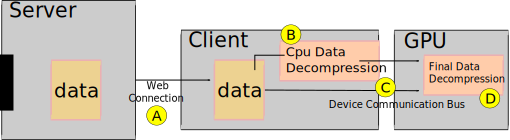
\includegraphics[width=\textwidth]{Immagini/genericdecompressionpipeline}
\caption[Schema agenti della distribuzione dei dati]{Schema degli agenti coinvolti nella distribuzione dei dati tridimensionali via rete. Sono posti in evidenza: A)la connessione di rete attraverso cui client e server comunicano; B)la ``decompressione'' effettuata, se necessario, dalla cpu del client; C)il bus di comunicazione tra la memoria principale e la memoria della GPU; D)l'eventuale e ulteriore ``decompressione'' effettuata dalla GPU stessa.\label{f:genericdecompressionpipeline}} 
\end{center} 
\end{figure}

\subsection{Applicazioni orientate al Web 3D}
Con la diffusione di applicazioni web 3D questa prospettiva \`e destinata per\`o a cambiare dato che per i sistemi tradizionali l'utilizzo di una grande quantit\`a di dati rende non pi\`u trascurabili i tempi di reperimento e caricamento. 
Per ovviare a questo problema, le soluzioni pi\`u diffuse sono una, a volte drastica, diminuzione della qualit\`a visiva o al rilascio di client che necessitano di installazione da parte dell'utente e che memorizzano in locale tutti i dati grafici. Quest'ultimo metodo \`e probabilmente il pi\`u diffuso per tutte quelle applicazioni che puntano ad avere sia elevata qualit\`a visiva che interazione tra utenti remoti, ma \`e anche quello che si separa di pi\`u dalle caratteristiche del web.
L'approccio del framework \`e invece quello di affrontare il problema aumentando la criticit\`a delle fasi di \textbf{accesso}, \textbf{costruzione e inizializzazione}.

Se si analizzano le applicazioni di grafica distribuite sulla rete, si pu\`o risalire a tre moduli distinti che sono di interesse: il server, il client e l'acceleratore grafico a disposizione del client. I dati contenuti sul server, per essere utilizzati, devono arrivare all'acceleratore grafico nella forma delle strutture dati proprie di quest'ultimo. Escludendo l'approccio a client con dati grafici autonomi possiamo modellizzare questo scenario come mostrato nella figura \ref{f:genericdecompressionpipeline}, in essa possiamo vedere in ordine temporale da sinistra a destra, il percorso fisico attraversato dai dati. Questi partono dal server e viaggiano attraverso una connessione web (A) fino a raggiungere il client, qui vengono caricati in memoria ed eventualmente ``decompressi'' dalla cpu (B), successivamente vengono inviati alla memoria video attraverso il bus di connessione della scheda grafica (C) ed infine, prima di essere visualizzati, possono dover attraversare un ulteriore processo di elaborazione/decompressione da parte della \ac{GPU} stessa (D). \`E facile identificare nella connessione (A) il collo di bottiglia del sistema, dato che in esso la banda a disposizione per il trasferimento dati \`e in assoluto la pi\`u piccola e non consente di sfruttare pienamente le capacit\`a di calcolo della \ac{GPU}.

Le applicazioni tradizionali si limitano ad utilizzare strutture dati datate, solitamente basate sulle mesh di vertici\footnote{Le mesh di vertici, o mesh poligonali, rappresentano i modelli tridimensionali attraverso un elenco di punti che definiscono i vertici di figure poligonali, di solito triangoli, in uno spazio tridimensionale.}, che per le loro caratteristiche producono file di grosse dimensioni, pi\`u che sufficienti nel caso in cui i dati sono memorizzati in locale, ma poco adeguati ad un contesto di comunicazione remota. I file vengono trasferiti attraverso il canale (A), il client se necessario effettua in (B) una decompressione dei dati e carica in memoria le informazioni contenute , nello stadio (C) i dati vengono trasferiti nella memoria video all'interno di strutture dati adatte a seconda del caso. Una volta all'interno della memoria della \ac{GPU} di solito i dati non vengono ulteriormente processati prima della visualizzazione, ma tutti gli ulteriori effetti vengono aggiunti durante il rendering stesso.

Dato il collo di bottiglia della connessione web (A) \`e proprio la dimensione dei file a rappresentare il maggiore limite del sistema. Per questo motivo \`e consuetudine che anche le applicazioni che non usano client con dati grafici preinstallati dedichino una fase iniziale ad effettuare il download completo di tutti i dati.

Le applicazioni basate sul modello del live streaming hanno problemi simili: in questo caso si ha il trasferimento attraverso (A) dei dati del flusso video, la banda occupata da questo flusso per livelli di qualit\`a medio-alta pu\`o variare da pochi Mbit/s alle decine di Mbit/s. Le informazioni video hanno bisogno di un solo stadio di decompressione che pu\`o essere effettuato sia direttamente dalla cpu in (B) che all'interno di processori grafici che implementano i decoder specifici, ma la \ac{GPU} vera e propria non viene affatto utilizzata. Come gi\`a accennato il vantaggio di ci\`o consiste nel fatto che il client non necessita affatto di avere a disposizione una \ac{GPU} e non vi \`e necessit\`a perci\`o di memorizzare i dati grafici. Gli svantaggi sono che vi \`e la necessit\`a di una connessione costante anche quando vengono visualizzati oggetti precedentemente visti e che la qualit\`a non \`e influenzata dall'hardware a disposizione, ma solo dalla banda a disposizione.

In entrambe le situazioni analizzate la possibilit\`a offerte dallo stadio (D) non vengono sfruttate ed \`e proprio tramite il suo utilizzo che lo Shadow Framework cerca di risolvere il problema. Facendo riferimento alla figura \ref{f:genericdecompressionpipeline}, sul server sono memorizzati i dati modellizzati in una forma parametrica adatta ad essere processata dalla \ac{GPU}: si pensi ad esempio ad una sfera descritta dalla posizione del proprio centro e dal suo raggio, utilizzando l'equazione parametrica della sfera \`e possibile calcolare dinamicamente in un secondo tempo la mesh di vertici che approssima il modello. Questa forma di ``decompressione'' dei dati consente di alleggerire i modelli contenuti nei file dal compito di trasportare al loro interno molte informazioni in maniera esplicita in maniera simile a quanto avviene ai formati vettoriali per le immagini bidimensionali. I file possono perci\`o essere di dimensioni contenute, diminuendo sensibilmente il tempo di \textbf{accesso} ai dati e scaricando parte del processo di reperimento delle informazioni anche sulla fase di \textbf{costruzione e inizializzazione} eseguita sulla \ac{GPU} stessa.

\subsection{Funzionalit\`a avanzate}
Alla luce del principio esposto al precedente paragrafo si pu\`o giungere successivamente ad ulteriori rielaborazioni di diverse pratiche sfruttate attualmente dai framework e dalle applicazioni grafiche. Una di queste pratiche \`e l'utilizzo della \textbf{precomputazione}, ovvero il processo di pre-calcolare dati computazionalmente troppo onerosi per essere gestiti in real-time. Questa precomputazione pu\`o essere eseguita in fase di inizializzazione di un'applicazione oppure essere effettuati a monte e memorizzati in modo statico in file la cui dimensione pu\`o rivelarsi. 

In contesto web la seconda soluzione \`e la meno conveniente dato che aumenta la quantit\`a di dati da trasferire attraverso il canale di comunicazione, ma alla luce dei moderni hardware grafici in generale anche la prima pu\`o essere ripensata sia nel senso di limitarla che nel senso di spostarne il peso computazionale direttamente sulla \ac{GPU}.

Un'altra interessante considerazione riguarda la valutazione del livello di dettaglio: le applicazioni tradizionali per adattare la qualit\`a delle immagini prodotte alla potenza dell'hardware a disposizione ricorrono all'espediente di fornire differenti varianti della stessa risorsa grafica a diversi livelli di qualit\`a. Per il rendering della stessa scena sono perci\`o disponibili modelli tridimensionali con un diverso numero di vertici o varianti della stessa immagine a diverse risoluzioni. Questo consente di alleggerire il calcolo su \ac{GPU} meno potenti, ma dato che aumenta notevolmente la dimensione dei dati \`e una soluzione insoddisfacente nel contesto web. L'utilizzo di una modellizzazione gerarchica all'interno del framework fornisce un meccanismo alternativo per gestire il livello di dettaglio che non va ad impattare sulla dimensione dei dati.

\begin{figure}
\begin{center}
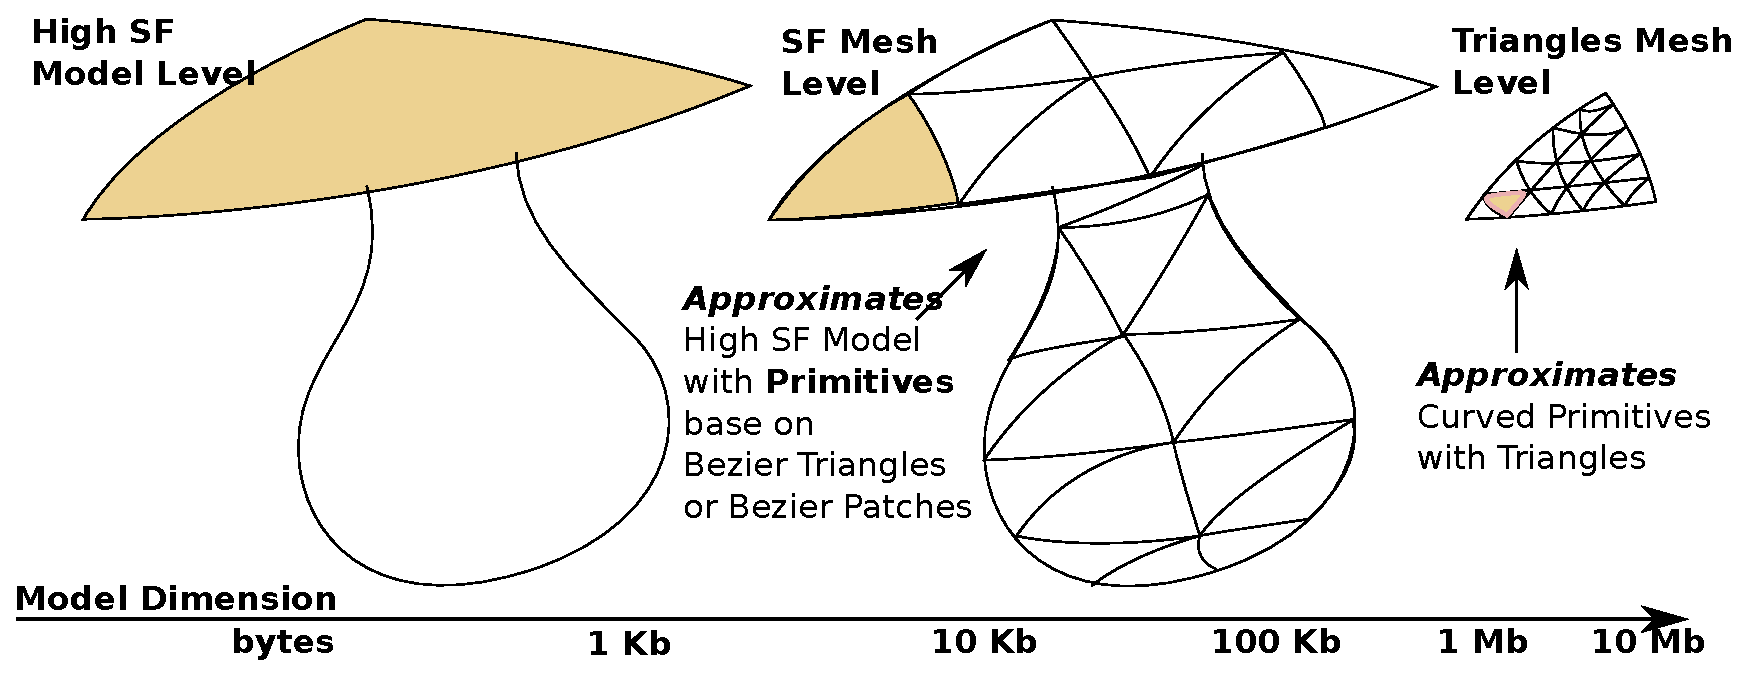
\includegraphics[width=\textwidth]{Immagini/hierarchicalmodeling}
\caption{Grafico della modellizzazione gerarchica del framework.\label{f:hierarchicalmodeling}} 
\end{center} 
\end{figure}

In figura \ref{f:hierarchicalmodeling} possiamo vedere come questa gerarchizzazione sia strutturata a due vie: sulla sinistra vediamo l'oggetto modellizzato ad alto livello, i file sf del framework contengono i dati riferiti a questo livello di astrazione che risultano molto compatti (dai pochi kbyte a qualche decina), ma comunque ricchi di informazioni.
La prima decompressione delle informazioni consiste nel tassellare\footnote{La tassellazione \`e un processo attraverso cui una superficie viene suddivisa in poligoni non sovrapposti.\cite{book:realtimerendering}} il modello parametrico con primitive di alto livello adatte allo scopo, in figura sono citati i triangoli di Bezier e le patch di Bezier. I dati estratti da questa prima fase possono raggiungere le centinaia di \ac{kB}. La seconda fase consiste in una ulteriore tassellazione delle primitive di alto livello in triangoli veri e propri che approssimano le superfici curve delle precedenti primitive e che possono essere usati direttamente della \ac{GPU} per effettuare il rendering. Questa operazione genera quantit\`a di dati la cui dimensione pu\`o essere anche di decine di \ac{MB}, ma essendo eseguita direttamente all'interno della memoria grafica il trasferimento ne risulta alleggerito. Il valore aggiunto di questa gerarchizzazione \`e che sfruttando su pi\`u livelli i processi di tassellazione ha intrinsecamente al suo interno un modo per scalare il livello di dettaglio modificando la granularit\`a della tassellazione stessa, evitando la duplicazione dei dati.

\subsection{Considerazioni finali sul framework}
La naturale premessa, essenziale per supportare le valutazioni espresse nei precedenti paragrafi, corrisponde alla necessit\`a da parte del framework di utilizzare un set di strutture geometrie intelligenti adatte allo scopo. Questo set deve soddisfare una serie di requisiti fondamentali senza i quali il framework incontrerebbe serie problematiche di applicabilit\`a e usabilit\`a, questi requisiti sono:
\begin{itemize}
	\item  la \textbf{completezza}, ovvero deve essere in grado di rappresentare ogni tipo di superficie del mondo reale;
	\item  la \textbf{semplicit\`a}, in quanto un set troppo complesso e articolato renderebbe il processo di selezione delle geometrie problematico;
	\item  la \textbf{flessibilit\`a}, nel senso che le geometrie devono essere in grado di scalare efficacemente in qualit\`a per venire incontro alle capacit\`a di apparecchiature differenti.
\end{itemize}

Questo \`e uno degli aspetti di ricerca e sperimentazione pi\`u interessanti del framework che, sebbene sia gi\`a sufficientemente maturo, \`e attualmente oggetto di ulteriore sviluppo.

\section{Struttura dello Shadow Framework 2.0}
\label{sec:sfstructure}
\begin{figure}
\begin{center}
\includegraphics[width=10cm]{Immagini/sfstructure}
\caption{Struttura dei moduli del framework.\label{f:sfstructure}} 
\end{center} 
\end{figure}
Il framework \`e strutturato in moduli gerarchici e la figura \ref{f:sfstructure} ne illustra i livelli e le loro dipendenze. Il livello pi\`u basso \`e quello denominato \textbf{system} e contiene al suo interno le astrazioni base sfruttate da tutti gli altri moduli. Ad un livello superiore troviamo il modulo \textbf{data} che si occupa di tutti gli aspetti riguardanti la gestione dati all'interno del framework. Per raggiungere gli obbiettivi prefissati il progetto di tesi \`e incentrato sull'estensione delle funzionalit\`a di questo livello e il capitolo \ref{ch:gestionedati} offre un approfondimento su meccanismi e le astrazioni su cui \`e fondato. Il livello \textbf{graphics} offre un'astrazione su di una pipeline di rendering ideale di cui possiamo osservare una rappresentazione in figura \ref{f:sfpipeline}. Dato che non esiste una implementazione diretta di questa pipeline, il framework la realizza configurando una pipeline programmabile attraverso l'\ac{API} OpenGL a cui si interfaccia tramite il modulo \textbf{graphics OpenGL}.
\begin{figure}
\begin{center}
\includegraphics[width=\textwidth]{Immagini/Pipeline}
\caption{Rappresentazione della pipeline ideale implementata dal framework.\label{f:sfpipeline}} 
\end{center} 
\end{figure}
Al di sopra del modulo graphics vi \`e \textbf{rendering}, che contiene il rendering engine vero e proprio che basa il suo funzionamento sulle caratteristiche della pipeline astratta del livello inferiore.
Il livello \textbf{rendering data} definisce infine la struttura dei dati grafici, questa struttura dipende dai livelli inferiori perch\`e deve tenere conto del modulo data per quanto concerne il reperimento dei dati, e del modulo rendering per i meccanismi di costruzione dei dati.

Le applicazioni costruite basandosi sul framework non hanno necessità di operare direttamente sulle \ac{API} grafiche a basso livello, ma possono essere strutturate per lavorare sulle astrazioni di alto livello offerte dal framework.

La versione del framework di riferimento, nonch\`e quella oggetto di sviluppo in questo progetto di tesi, \`e quella realizzata in linguaggio Java e disponibile tramite la fonte indicata al paragrafo \ref{sub:sfsource}. 
Per questa versione il modulo \textbf{graphics OpenGL} non si interfaccia direttamente con le \ac{API} OpenGL, ma sfrutta a tal scopo la libreria del progetto JOGL\footnote{Per informazioni sulla libreria JOGL fare riferimento al paragrafo \ref{sub:jogl}.}.
